\documentclass[border=10pt]{standalone}

\usepackage{tikz}
\usepackage{tikzsymbols}
\usetikzlibrary{calc,patterns,shapes.geometric}

\def\centerarc[#1](#2)(#3:#4:#5){\draw[#1] ($(#2)+({#5*cos(#3)},{#5*sin(#3)})$) arc (#3:#4:#5);}

\begin{document}
	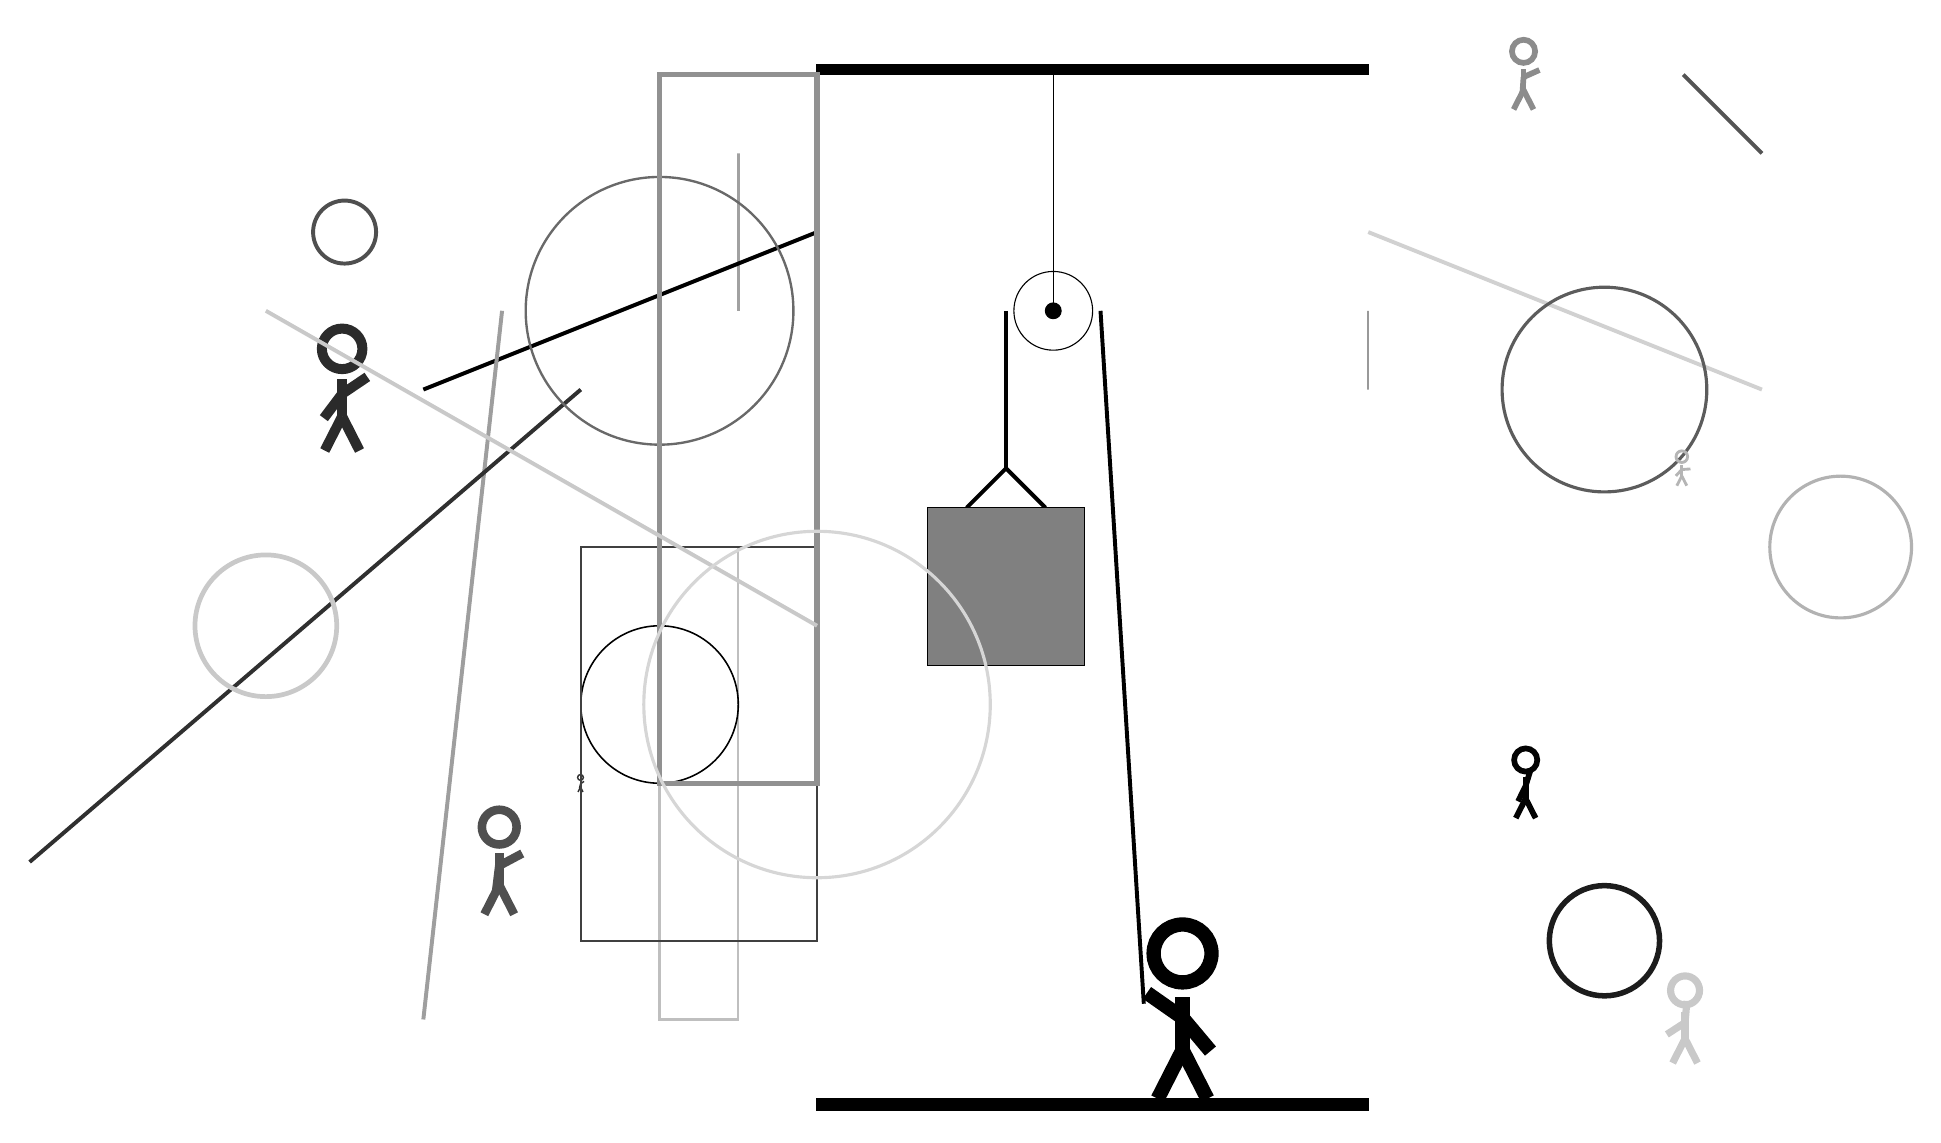
\begin{tikzpicture}
		%%%%% START %%%%%
		
		\draw[fill=black] (-2, 10) rectangle (5, 10.125);
		
		\draw (1, 7) circle (0.5);
		\draw[fill=black] (1, 7) circle (0.1);
		\draw (1, 10) -- (1, 7);
		
		\draw[line width=0.5mm] (-0.1, 4.5) -- (0.4, 5.0) -- (0.9, 4.5);
		\draw[fill=black!50] (-0.6, 4.5) rectangle (1.4, 2.5);
		
		\draw[line width=0.5mm] (0.4, 7) -- (0.4, 5.0);
		\centerarc[line width=0.5mm](1, 7)(0:180:0.6);
		\draw[line width=0.5mm](1.6, 7) -- (2.15, -1.8);
		
		\node at (2.6, -1.9) {\Strichmaxerl[10][-35][-50]};
		
		\draw[line width=0.2mm, color=black!40] (5, 6) rectangle (5, 7);
		
		\draw [line width=0.4mm, color=black!30](11, 4) circle (0.9);
		\node[line width=0.4mm, color=black!81] at (-5, 1) {\Strichmaxerl[1][77][35]};
		\node[line width=0.7mm, color=black!69] at (-6, 0) {\Strichmaxerl[6][83][28]};
		\draw[line width=0.4mm, color=black!37] (-3, 9) rectangle (-3, 7);
		
		\draw[line width=0.5mm, color=black!67](10, 9) -- (9, 10);
		\node[line width=0.2mm, color=black!99] at (7, 1) {\Strichmaxerl[4][64][73]};
		\node[line width=0.2mm, color=black!83] at (-8, 6) {\Strichmaxerl[7][53][34]};
		\draw[line width=0.3mm, color=black!25] (-4, -2) rectangle (-3, 4);
		\draw [line width=0.7mm, color=black!89](8, -1) circle (0.7);
		\node[line width=0.2mm, color=black!45] at (7, 10) {\Strichmaxerl[4][86][24]};
		\draw[line width=0.5mm, color=black!100](-2, 8) -- (-7, 6);
		\draw [line width=0.2mm, color=black!100](-4, 2) circle (1.0);
		\draw[line width=0.5mm, color=black!18](10, 6) -- (5, 8);
		\draw[line width=0.2mm, color=black!75] (-2, 4) rectangle (-5, -1);
		\draw [line width=0.4mm, color=black!64](8, 6) circle (1.3);
		
		\draw[line width=0.5mm, color=black!38](-6, 7) -- (-7, -2);
		\draw[line width=0.5mm, color=black!81](-5, 6) -- (-12, 0);
		\draw [line width=0.6mm, color=black!21](-9, 3) circle (0.9);
		
		\draw [line width=0.5mm, color=black!69](-8, 8) circle (0.4);
		\draw [line width=0.3mm, color=black!59](-4, 7) circle (1.7);
		
		\node[line width=0.3mm, color=black!29] at (9, 5) {\Strichmaxerl[2][47][4]};
		
		\draw[line width=0.7mm, color=black!43] (-2, 1) rectangle (-4, 10);
		\node[line width=0.3mm, color=black!21] at (9, -2) {\Strichmaxerl[5][33][85]};
		\draw[line width=0.5mm, color=black!21](-2, 3) -- (-9, 7);
		
		\draw [line width=0.4mm, color=black!16](-2, 2) circle (2.2);
		
		\draw[fill=black] (-2, -3) rectangle (5, -3.15);
		
		%%%%% END %%%%%
	\end{tikzpicture}
\end{document}